% !TeX root = ../../Thesis.tex
\chapter{Effects of an External Magnetic Field on Stimulated Raman Scattering}
\label{chp:magSRS}

In this chapter, we present work performed by the author while employed as a Junior Specialist at the University of California, San Diego between January and April 2020. The project was supervised by Professor Farhat Beg, and lead by Adam Higginson (\href{https://orcid.org/0000-0002-2727-8075}{ORCID: 0000-0002-2727-8075}). The work presented (including data generated and data analysis) was carried out by the author, except in the cases outline below:
\begin{itemize}
\item Figure \ref{fig:SRS_LULI} was produced by M. Bailly-Grandvaux (\href{https://orcid.org/0000-0001-7529-4013}{ORCID: 0000-0001-7529-4013}).
\end{itemize}

The chapter begins with a review of the literature which discusses the effect of an externally-applied magnetic field on stimulated Raman scattering. We then present modelling, performed by the author, of an experiment performed at the \acrlong{LULI} (France): J. R. Marqu\`es, P. Loiseau, J. B\'eard, A. Castan, B. Coleman, T. Gangolf, L. Lancia, A. Soloviev, O. Portugall, and J. Fuchs. Analysis of the SRS diagnostics was performed by J. R. Marq\`es, and (revisited) by M. Bailly-Grandvaux.  The experiment showed a small increase in SRS with an applied magnetic field, and this is recreated in our simulations. We then go on to investigate how the effect of the magnetic field depends on $\kld$ of the SRS electron plasma wave.

\section{Motivation and literature review}


Once again, wjhy is this a problem? why can we model in 1D? 

How can we continue to only consider modes without B field? Why no X or O modes?

GREAT PAPER it's fluid theory of SRS SBS competition in magnetised plasmas\citep{Vyas2016}

\subsection{Magnetic field suppresses kinetic SRS}

An electron plasma wave (\acrshort{EPW}) which propagates perpendicularly to a magnetic field experiences damping, caused by the trapped electrons being accelerated across the EPW wave-front and extracting energy from it \citep{Dawson1983}. As was introduced in Chapter \ref{chp:theory}, inflationary stimulated Raman scattering (\acrshort{iSRS}), which takes place in a homogeneous plasma, depends on the damping of the EPW .

The first step of this research project was to replicate the results of \citet{Winjum2018}, in order to benchmark the EPOCH code against the results from OSIRIS and to understand the relevant diagnostics. Figure \ref{fig:WinjumRep} demonstrates the main results of replicating \citet{Winjum2018}. The simulations summarised in Figure \ref{fig:WinjumRep} consider homogeneous SRS in the kinetic regime, with and without a $30\si{T}$ magnetic field applied parallel to the polarisation of the laser. By comparing the left ($B_{\text{ext}}=0\si{T}$) and right ($B_{\text{ext}}=30\si{T}$) columns of Figure \ref{fig:WinjumRep}, we see three key features of the simulation: sub-figures (a) and (b) show that the convective growth of SRS EPWs is suppressed by the magnetic field; sub-figures (c) and (d) show that the population of electrons trapped in the SRS EPWs becomes de-trapped by the magnetic field; sub-figures (e) and (f) show that the magnetic field introduces a periodic disturbance to the electron trapping, and accelerates electrons to with positive and negative $x$-momenta. Recalling the definition of the cyclotron frequency, we can calculate that for a $30\si{T}$ external magnetic field, $\omega_c = eB_0/m_e = 5 \times 10^{12}$ $\si{rad}\si{s}^{-1}$. From inspection of Figure \ref{fig:WinjumRep} (e)

A 2021 paper by \citet{Zhou2021} uses 1D and 2D \acrshort{PIC} simulations to show that a moderate external magnetic field can suppress inflationary SRS, so that the SRS reflectivity stays at its convective saturation level from fluid theory. 



\begin{figure}[ht]
   \centering
    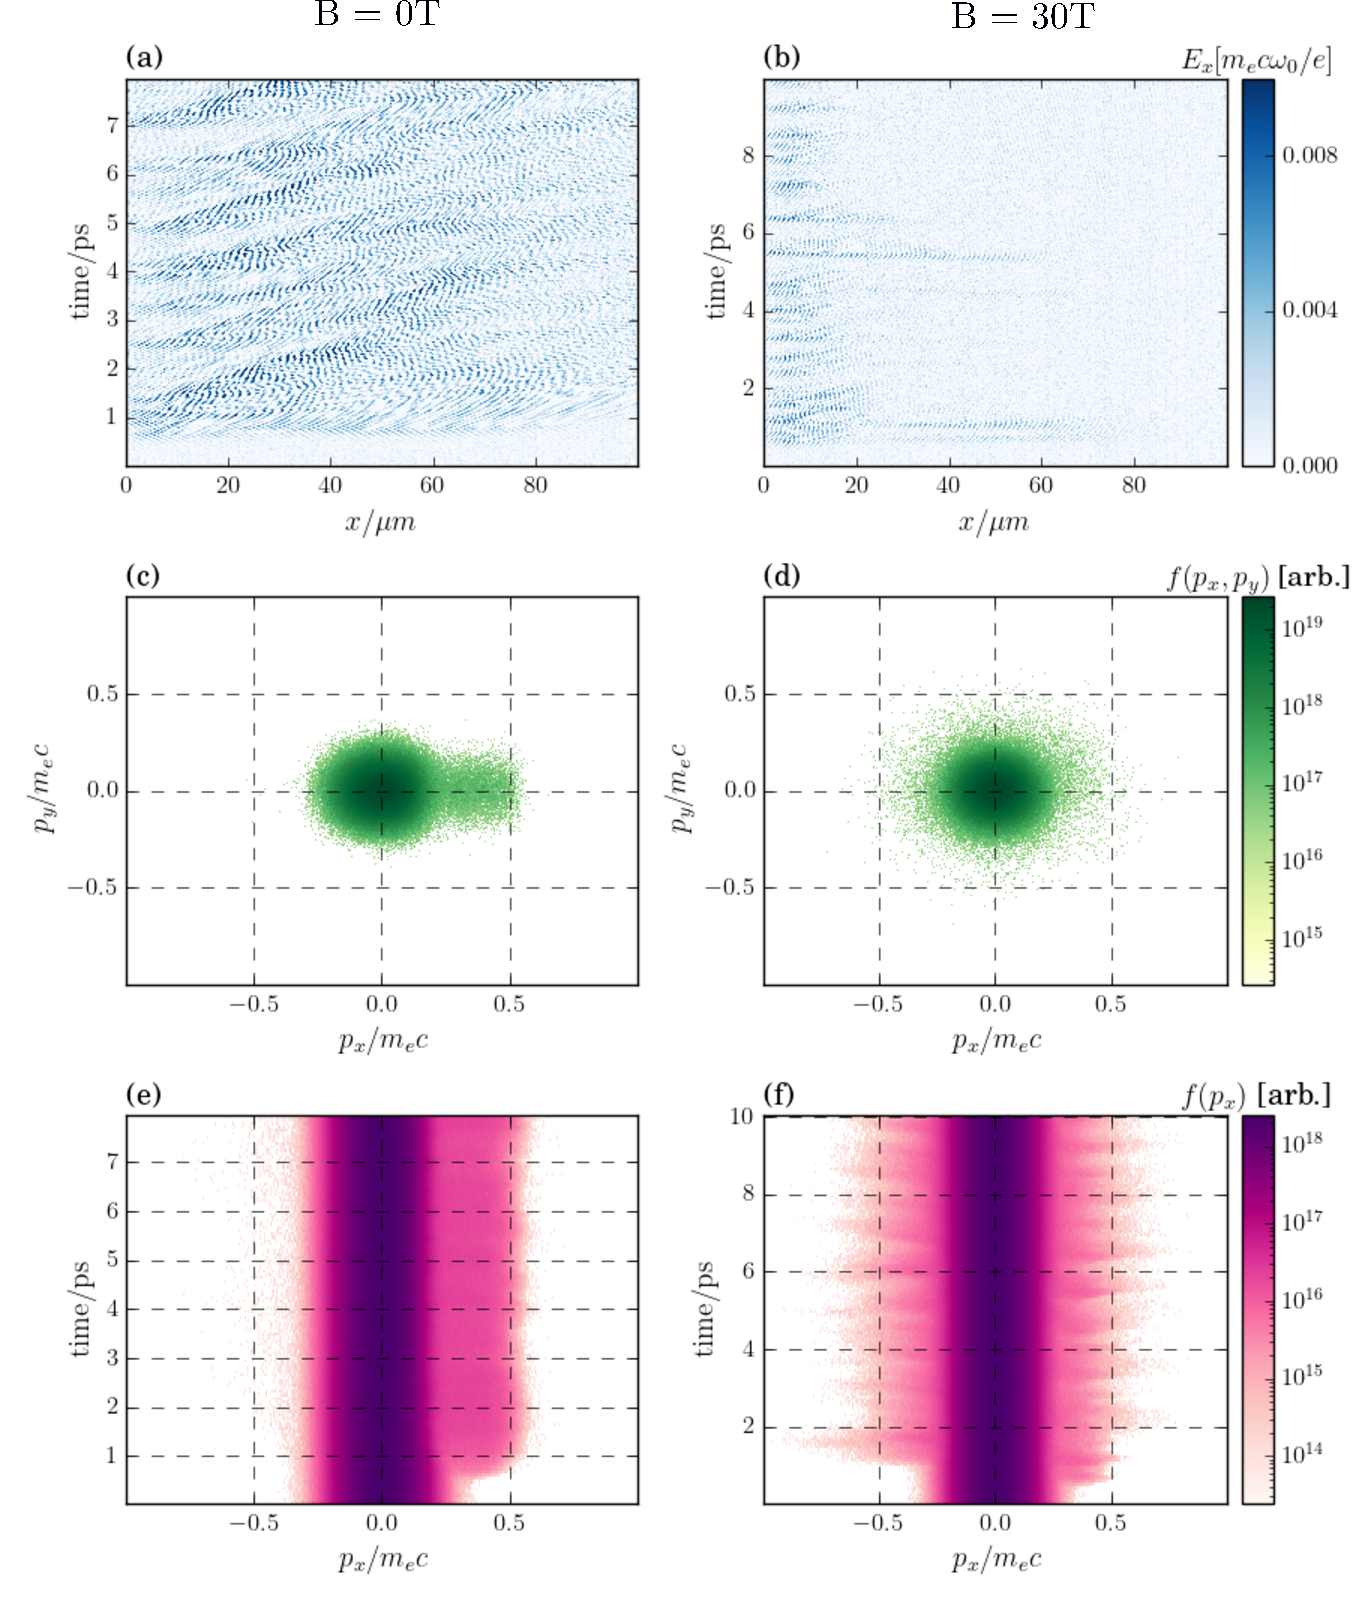
\includegraphics[width=\columnwidth]{Chapters/C6_magSRS/Winjum_rep_megaPlot_label.pdf}
    \caption{Comparison of the key diagnostics with different external magnetic fields: 0T (left column) and 30T (right column). The first row (sub-figures a,b) shows the electrostatic ($E_x$) fields as a function of space and time. The second row (sub-figures c,d) shows the $p_x,p_y$ distribution functions averaged over space, at $t=T_{\mathrm{end}}$. The final row (sub-figures e,f) shows the $p_x$ distribution, averaged over space, as a function of time. Simulation parameters chosen for comparison with Figure 2b of \citet{Winjum2018}.}
    \label{fig:WinjumRep}
\end{figure}{}




\subsection{Magnetic field could enhance kinetic SRS}

\subsection{What about fluid SRS?}

\begin{figure}[ht]
   \centering
    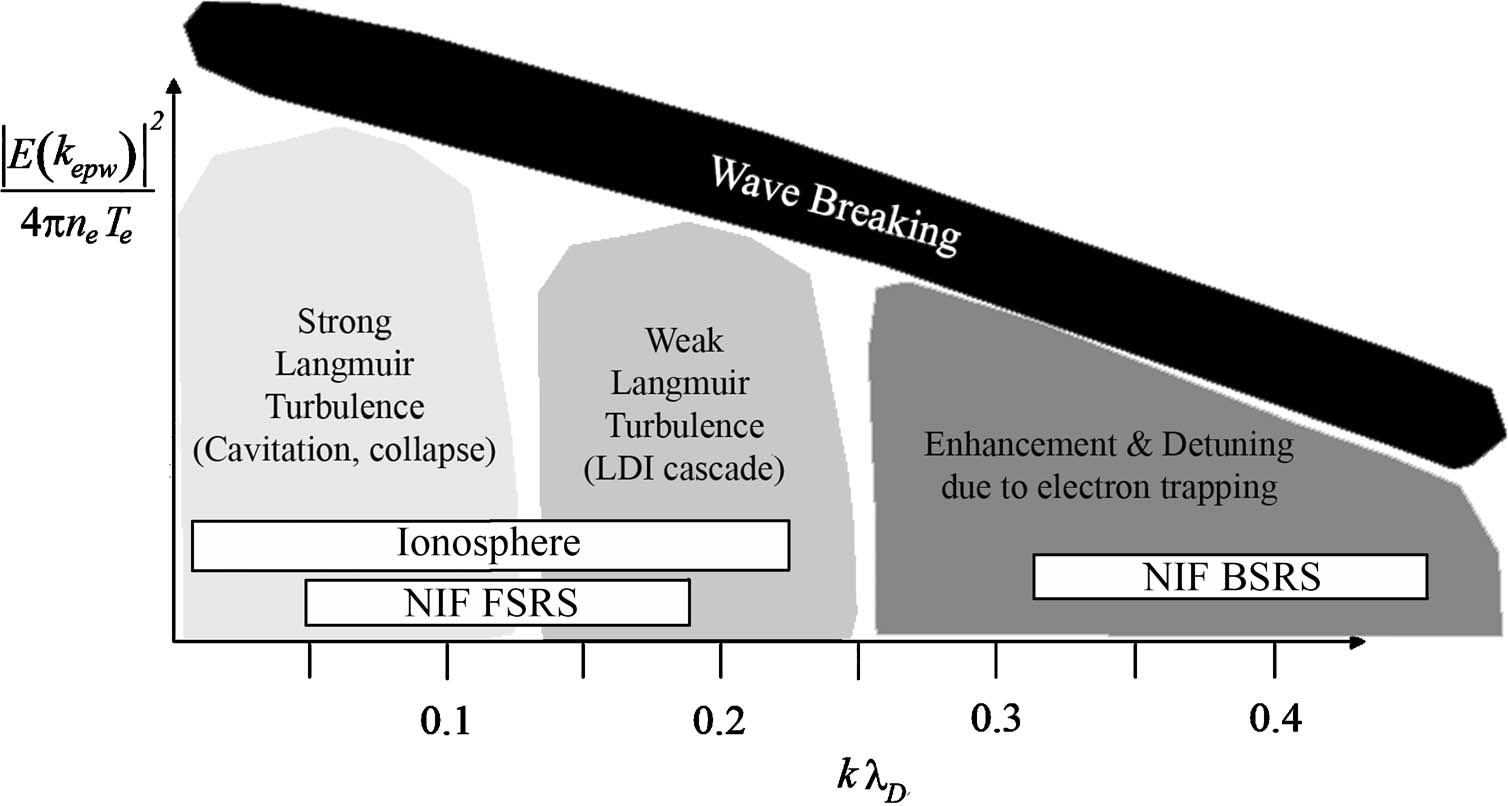
\includegraphics[width=\columnwidth]{Chapters/C6_magSRS/kld_regimes.png}
    \caption{Pictoral view of different non-linear regimes for \acrshort{EPW}s as a function of $\kld$. Reprinted with permission from \citet{Kline2006} (re-use license in Appendix 1).}
    \label{fig:Kline2006}
\end{figure}{}


In the fluid regime, electron trapping, and de-trapping by the magnetic field, is no longer the most important factor in the nonlinear evolution of the \acrshort{SRS} \acrshort{EPW}. Consulting \citet{Kline2006}'s paper ``Different $\kld$ regimes for nonlinear effects on Langmuir waves", we see that 

\section{Modelling SRS on LULI}
\subsection{Experimental results}
\begin{figure}[ht]
   \centering
    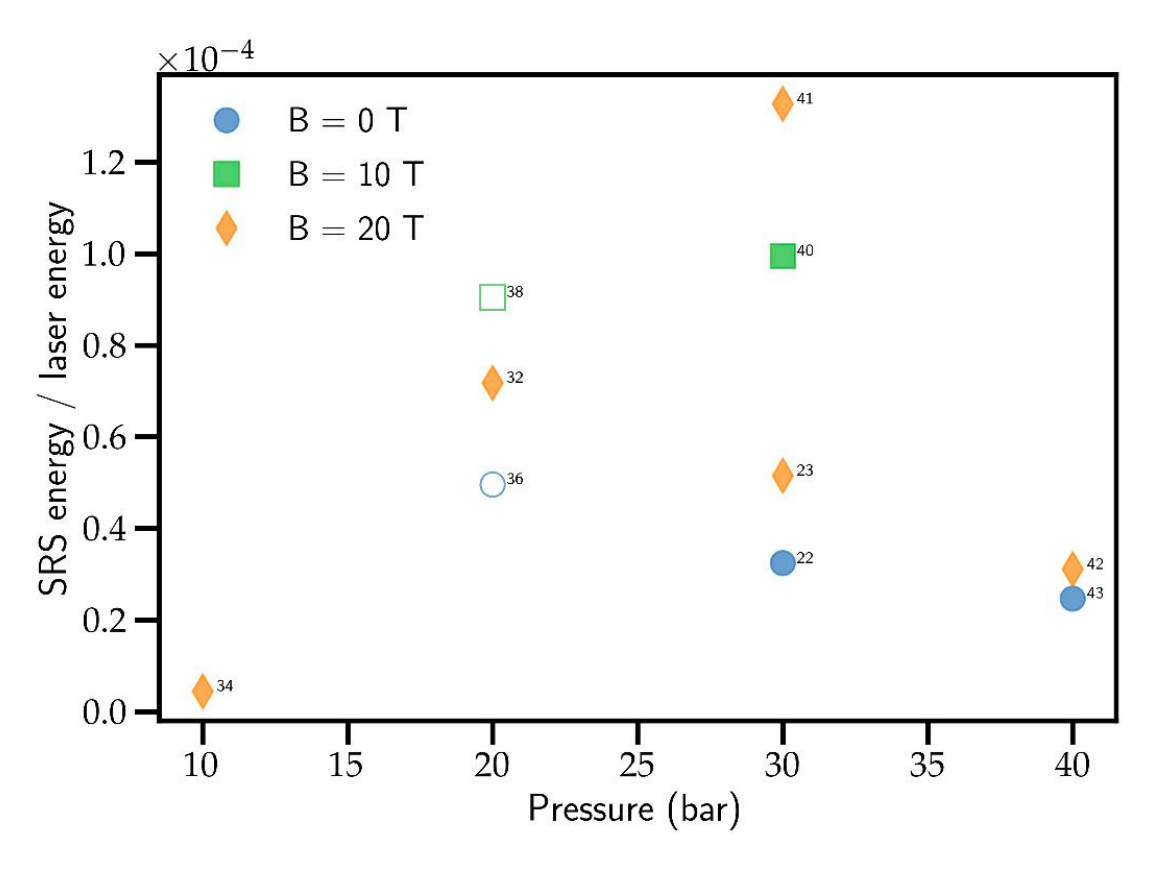
\includegraphics[width=0.8\columnwidth]{Chapters/C6_magSRS/SRS_LULI.png}
    \caption{\textbf{Figure produced by M. Bailly-Grandvaux.} Experimentally-measured SRS energy at different gas jet pressures, with and without magnetic fields. The solid-coloured markers represent shots with the laser  horizontally polarised with respect to the applied magnetic field, so that the laser magnetic field and applied magnetic field are parallel. The un-filled markers represent vertical polarisation of the laser.}
    \label{fig:SRS_LULI}
\end{figure}{}


\subsection{Simulation results}

Plasma density and temperature profiles at the centre of the gas jet were simulated using the FLASH code by Adam Higginson. 

\begin{table}[h]
\begin{center}

\begin{tabular}{|l|l|l|l|}
\hline
$n_e$ / $n_{\mathrm{cr}}$ & $T_e$ / eV & bSRS $\kld$ & fSRS $\kld$\\ \hline \hline
0.01 & 180 & 0.36 & 0.02 \\ \hline
0.025& 450 & 0.34 & 0.03 \\ \hline
0.05 & 600 & 0.27 & 0.04 \\ \hline
0.10 & 900 & 0.21 &  0.05\\ \hline
0.15 & 1100 & 0.18 & 0.06 \\ \hline

\end{tabular}

\end{center}
\caption{$T_i$ is $T_e/3$ in all cases}
\label{tab:LULI_setup}
\end{table}


\begin{figure}[ht]
   \centering
    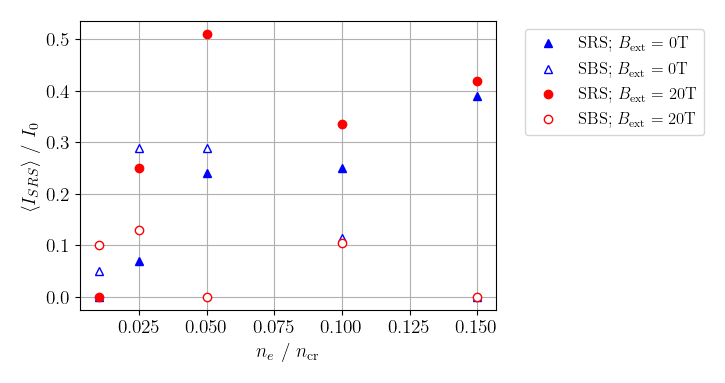
\includegraphics[width=\columnwidth]{Chapters/C6_magSRS/LULI_sims_v3.png}
    \caption{Reflected light from SRS and SBS (averaged over full simulation time) as a function of the initial homogeneous plasma density. Plasma densities and temperatures taken from FLASH simulations of single-beam shots without magnetic fields. The range of $\kld$ probed is 0.36, 0.34, 0.27, 0.21, 0.18.}
    \label{fig:LULI_sims_v3}
\end{figure}{}



\section{Magnetic field effect varies with plasma debye length}

\citep{Feng2018} REALLY good reference about SRS and LDI and anti-LDI

also don't forget this great paper about kld scling of iSRS autoresonance \citep{Chapman2013}

\subsection{Fixed ions: vary $\kld$}

\begin{figure}[ht]
   \centering
    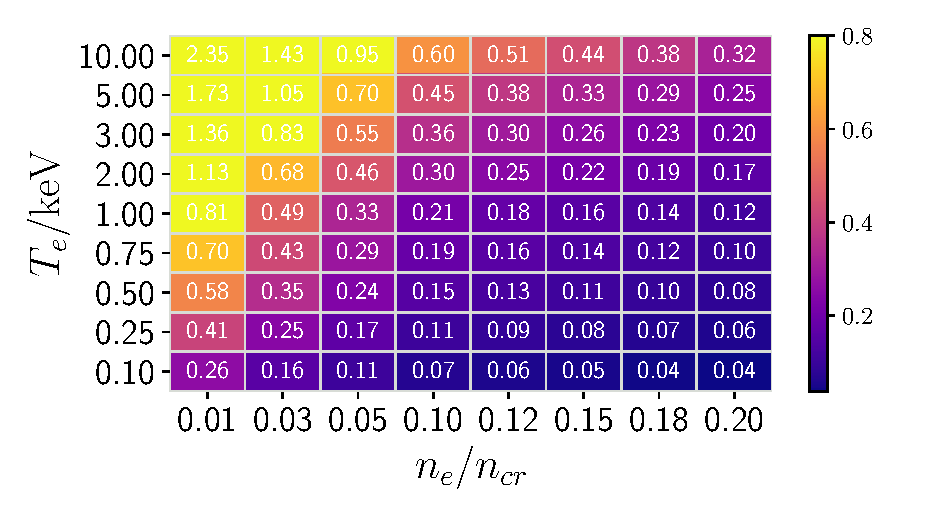
\includegraphics[width=\columnwidth]{Chapters/C6_magSRS/kld_scan_ben_simon.pdf}
    \caption{calculations innit}
    \label{fig:kld_scan}
\end{figure}{}

WHAT IS cyclotron frequency / wpe for all these cases?

Plasma parameters chosen to be relevant to LULI experiment (ish). $\lambda_0 = 1053 \si{\nano\metre}$; $L_x = 1000 \si{\micro\metre}$; $T_e = 1 \si{\kilo\electronvolt}$; $I_0 = 1\times 10^{15}\si{W/\cm^2}$; $T_{\mathrm{end}}=10 \si{ps}$; 1000 PPC (from convergence testing on $\left< I_{\mathrm{SRS}} \right>_{t>0}$).

\begin{table}[h]
\begin{center}

\begin{tabular}{|l|l|l|l|}
\hline
$n_e$ / $n_{\mathrm{cr}}$ & $\kld$ & regime & predicted behaviour\\ \hline \hline
0.02 & 0.55 & beyond ``loss of resonance" & no SRS, no dependence on $B_{\mathrm{ext}}$  \\ \hline
0.05 & 0.33 & strongly kinetic &  \\ \hline
0.08 & 0.25 & kinetic &  \\ \hline
0.11 & 0.20 & weakly kinetic & \\ \hline
0.20 & 0.12 & fluid & no dependence on $B_{\mathrm{ext}}$\\ \hline

\end{tabular}

\end{center}
\caption{Plasma density, $\kld$, regime, predicted behaviour}
\label{tab:predictions}
\end{table}

\begin{figure}[ht]
   \centering
    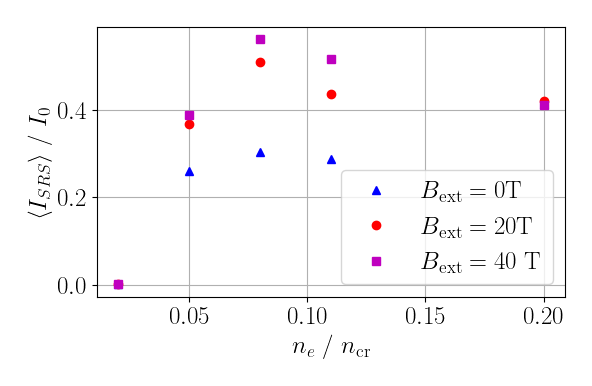
\includegraphics[width=0.9\columnwidth]{Chapters/C6_magSRS/kld_scan_SRS_scaling.png}
    \caption{Reflected light from SRS, averaged over the full simulation time, as a function of the initial homogeneous plasma density. By fixing the temperature at $T_e = 1\si{\kilo\electronvolt}$, the folowing values of $\kld$ are probed: 0.55, 0.33, 0.25, 0.20, 0.12. The following parameters are constant to all the simulations: 
 $\lambda_0 = 1056 \si{\nano\metre}$; $L_x = 1000 \si{\micro\metre}$; $T_e = 1 \si{\kilo\electronvolt}$; $I_0 = 1\times 10^{15}\si{W/\cm^2}$; $T_{\mathrm{end}}=10 \si{ps}$; 1000 PPC.}
    \label{fig:SRS_EPOCH}
\end{figure}{}


\section{Magnetic field effect changes with polarisation}

\section{Conclusion}



